\documentclass{scrartcl}

\usepackage{amsmath,amssymb,amsfonts}
\usepackage{graphicx}
\usepackage{subcaption} % Do not use subfigure.

\title{Unscented Kalman Filter (UKF) Highway Project}
\author{Philipp Rapp}
\date{\today}

\begin{document}

\maketitle

\section{UKF Algorithm}
The UKF algorithm has been presented in great detail in Lesson 04 of the Nanodegree.
I was able to reuse the code which I implemented in the quizzes.

Just like the regular Kalman filter (KF) and other types of observers, the UKF
has a predictor-corrector structure. Prediction is done with the plant model $f(x)$
(aka state transition probability), and correction (or measurement update) is done
with the measurement model $h(x)$.

Opposed to other flavors of KF, the state probability density function (PDF)
is represented by means of $\sigma$-points (which can be understood as
some sort of particles that have been chosen in a smart way).

\subsection{Prediction}
Our state vector is defined as
\begin{equation}
	x = \left( p_x, p_y, v, \psi, \dot{\psi} \right)^T \in \mathbb{R}^5
\end{equation}
with the Cartesian position $p_x$ and $p_y$ (in meter),
the speed (i.e., velocity magnitude) $v$ (in m/s),
the yaw angle $\psi$ (in radians),
and the yaw rate $\dot{\psi}$ (in rad/s).
Its dimension is $n_x = 5$.

The corresponding estimation error covariance matrix is $P \in \mathbb{R}^{5 \times 5}$.

\paragraph{Create augmented $\sigma$ points.}
We introduce the augmented state
\begin{equation}
	x_a = \left( p_x, p_y, v, \psi, \dot{\psi}, \nu_a, \nu_{\ddot{\psi}} \right)^T \in \mathbb{R}^7
\end{equation}
of dimension $n_a = 7$, which contains the regular states
and the (longitudinal) acceleration noise $\nu_a$ and yaw acceleration noise $\nu_{\ddot{\psi}}$.
Note that the mean values for the noise are 0.

We also create the augmented covariance matrix
\begin{equation}
	P_a = \left( \begin{array}{cc}
				P & 0 \\
				0 & Q
				\end{array} \right) \in \mathbb{R}^{n_a \times n_a}.
\end{equation}

Using Cholesky decomposition, we compute the lower triangular matrix $A_a$ such that
\begin{equation}
	A_a \cdot A_a^T = P_a
\end{equation}
With the spreading parameter
\begin{equation}
	\lambda = 3 - n_a = 3 - 7 = -4
\end{equation}
we compute the (augmented) sigma points
\begin{equation}
	\mathcal{X}_a = \left(
	x_{a,k|k} \qquad x_{a,k|k} + \sqrt{\lambda+n_a} A_a \qquad x_{a,k|k} - \sqrt{\lambda+n_a} A_a
	 \right) \in \mathbb{R}^{n_a \times n_\sigma}
\end{equation}
with $n_\sigma = 2 n_a + 1 = 2 \cdot 7 + 1 = 15$.

\paragraph{Predict the sigma points.}
Each of the $n_\sigma$ $\sigma$ points (i.e., every column in $\mathcal{X}$)
is predicted by means of the plant or state transition model, which represents the CTRV
(constant turn rate and velocity) model.
We get the predicted sigma points $X_{k+1|k} \in \mathbb{R}^{n_x \times n_\sigma}$.
Note that the number of rows changed from $n_a = 7$ to $n_x = 5$, as we
use the noise states only as input, but do not predict them.

\paragraph{Compute the state mean and the covariance.}
We compute $n_\sigma$ weights as
\begin{align*}
	w_i &= \frac{\lambda}{\lambda + n_a} \quad \text{for} \quad i=1, \\
	w_i &= \frac{1}{2 (\lambda + n_a)} \quad \text{for} \quad i=2,3,\dots,n_\sigma.
\end{align*}

We can then compute the predicted mean and covariance as
\begin{align*}
	x_{k+1|k} &= \sum_{i=1}^{n_\sigma} w_i X_{k+1|k, i} \\
	P_{k+1|k} &= \sum_{i=1}^{n_\sigma} w_i
			\left( X_{k+1|k, i}-x_{k+1|k} \right)
			\left( X_{k+1|k, i}-x_{k+1|k} \right)^T.
\end{align*}

\paragraph{Nomenclature.}
After the prediction, the state $x_{k+1|k}$ is called \emph{a priori}
(because it is \emph{before} we included any new data that
came from a measurement).

\subsection{Correction (measurement update)}

\subsubsection{Linear measurement model}
The lidar measurement model is linear and given by
\begin{equation}
	z_\text{L} = H_\text{L} \cdot x
\end{equation}
with
\begin{equation}
	H_\text{L} = \left( \begin{array}{ccccc}
		1 & 0 & 0 & 0 & 0 \\
		0 & 1 & 0 & 0 & 0
	\end{array} \right) \in \mathbb{R}^{2 \times 5}.
\end{equation}

The measurement is denoted by $z$, and the innovation is denoted by $y$.
The \emph{a priori} quantities are denoted by a prime.

The Lidar update equations are just like for the linear KF and given by
\begin{align*}
	y &= z - H_\text{L} \cdot x^\prime \\
	S &= H_\text{L} \cdot P^\prime \cdot H_\text{L}^T + R_\text{L} \\
	K &= P^\prime \cdot H_\text{L}^T \cdot S^{-1} \\
	x &= x^\prime + K \cdot y \\
	P &= \left( I - K \cdot H_\text{L} \right) \cdot P^\prime.
\end{align*}
The formulas are taken from Lesson 03 about the Extended Kalman Filter (EKF).

\subsubsection{Nonlinear measurement model}
The Radar measurement model is nonlinear.
For this reason, the predicted state $\sigma$ points $X_{k+1|k}$
are used for computing the measurement $\sigma$ points.

Those are used for the update step as given in Concepts 26 and 29 of Lesson 04.

Care needs to be taken to always normalize angles. That holds true for
the Radar bearing (or azimuth) angle $\phi$, as well as for the yaw angle $\psi$.

\paragraph{Nomenclature.}
After the correction or update, the state is called \emph{a posteriori}
(because it is \emph{after} we included the new information
from the measurement).

\section{Parameters}
A KF solves a (discrete-time) differential equation by integrating it.
Therefore, initial conditions $x_0$ and $P_0$
for the state $x$ and the estimation error
covariance matrix $P$ are required.

On top of that, we need covariance matrices which describe the
process noise $Q$ and the measurement noise $R$.
Whereas the latter are obtained from the sensor data sheet or
by evaluating the sensor noise, the former need to be estimated,
``guestimated'', or tuned in some way.

\subsection{Initial conditions}
The position is initialized by means of the first measurement
(be it Lidar or Radar).
In case of Lidar, which measures the Cartesian position, we use directly
\begin{align*}
	p_x &= p_x, \\
	p_y &= p_y.
\end{align*}
In case of Radar, we use
\begin{align*}
	p_x &= \rho \cos(\phi), \\
	p_y &= \rho \sin(\phi).
\end{align*}

I decided to not initialize any other components of the state with non-zero values,
not even the speed,
even though Radar measures the velocity,
That is because Radar yields the radial relative velocity,
but not the speed $v$ which is contained in the state.
It could even be the case that a car is moving tangentially (for instance
on a circle around our ego vehicle) with a high speed,
and still Radar measures a range rate $\dot{\rho}$ of (approximately) 0.

However, for this reason, I decided to initialize $P$ with large values
for all state components other than position.
I decided to use 2\,m standard deviation in the position (which is larger
than the Lidar uncertainty, but given that fact that the Cartesian uncertainty
of Radar increases with the range, 2\,m felt like an adequate initial uncertainty value).

For the speed, I chose 5\,m/s (which is 18\,kph) initial uncertainty.
For the yaw angle, I chose 180\,deg (corresponding to $\pi$), as we do not
know anything about it in the beginning.
Similarly, I chose 12\,deg/s (or 0.2\,rad/s) for the initial yaw rate uncertainty.


\subsection{Process noise}

The initial process noise standard deviations are given as
\begin{align*}
	\sigma_a &= 30\,\text{m}/\text{s}^2 \\
	\sigma_{\ddot{\psi}} &= 30\,\text{rad}/\text{s}^2 \, (= 1719\,\text{deg}/\text{s}^2)
\end{align*}
As state in Lesson 04, a rule of thumb is to set the standard deviation
to half of the maximum expected value.
Assuming $6\,\text{m}/\text{s}^2$ as the maximum acceleration, we should rather set
\begin{equation}
	\sigma_a = 3\,\text{m}/\text{s}^2.
\end{equation}
Similarly, assuming that a vehicle needs at least 4 seconds for performing a full
360 degree rotation, we get a maximum yaw rate of $2 \pi / 4\,\text{s} = 1.57\,\text{rad}/\text{s}$.
Assuming that a driver changes from one direction to the other within two seconds, we have
a yaw acceleration of $1.57\,\text{rad}/\text{s} / 2\,\text{s} \approx 0.8\,\text{rad}/\text{s}^2$.
We should therefore set the yaw acceleration noise to
\begin{equation}
	\sigma_{\ddot{\psi}} = 0.4\,\text{rad}/\text{s}^2 \, (= 22.9\,\text{deg}/\text{s}^2).
\end{equation}

\subsection{Measurement noise}
The lidar measurement noise standard deviations are given as
\begin{align*}
	\sigma_{p_x} &= 0.15\,\text{m}, \\
	\sigma_{p_y} &= 0.15\,\text{m}.
\end{align*}
The measurement noise covariance matrix is therefore
\begin{equation}
	R_\text{L} = \left( \begin{array}{ccc}
		\sigma_{p_x}^2 & 0 \\
		0 & \sigma_{p_y}
		\end{array} \right) \in \mathbb{R}^{2 \times 2}.
\end{equation}

The radar measurement noise standard deviations are given as
\begin{align*}
	\sigma_\rho &= 0.3\,\text{m}, \\
	\sigma_\phi &= 0.03\,\text{rad} \, (= 1.72\,\text{deg}), \\
	\sigma_{\dot{\rho}} &= 0.3\,\text{m/s}.
\end{align*}
The measurement noise covariance matrix is therefore
\begin{equation}
	R_\text{R} = \left( \begin{array}{ccc}
		\sigma_\rho^2 & 0 & 0 \\
		0 & \sigma_\phi^2 & 0 \\
		0 & 0 & \sigma_{\dot{\rho}}
		\end{array} \right) \in \mathbb{R}^{3 \times 3}.
\end{equation}

\section{Analysis}
As suggested in the lesson, I had a look into the normalized innovation squared (NIS).
This is done for the initial, unmodified process noise $Q$, as well as for
the adjusted process noise $Q$.

\subsection{Unmodified process noise}
For all three cars, the NIS
\begin{equation}
	y^T \cdot S^{-1} \cdot y
\end{equation}
has been evaluated. It is shown in Figure~\ref{fig:nis:default_process_noise}.
We see the histogram of the NIS value along with the expected $\chi^2$ distribution.

It can be seen that the Lidar update fits pretty well.
That makes sense, as the Lidar innovation only involves the position,
and because the involved position uncertainties are either given by the sensors itself,
or estimated by our UKF.

For the Radar update however, the NIS is too small.
That means that we overestimate the uncertainty of the predicted measurement.
Stated in another way, we put too much uncertainty in our estimated state
(which is used to compute the predicted or expected measurement).
That is probably due to a too large process noise, so we should decrease
the process noise $Q$.
It also makes sense that only the Radar update is affected, as it is
directly influenced by the process noise $Q$, which acts on the acceleration level
and therefore influences our velocity estimate.


\begin{figure}[!ht]
	\centering
	\begin{subfigure}[c]{0.45\columnwidth}
		\includegraphics[width=\textwidth]{%
			./img/nis_unmodified_process_noise/car1_lidar}
	\end{subfigure}
	\begin{subfigure}[c]{0.45\columnwidth}
		\includegraphics[width=\textwidth]{%
			./img/nis_unmodified_process_noise/car1_radar}
	\end{subfigure}
	\begin{subfigure}[c]{0.45\columnwidth}
		\includegraphics[width=\textwidth]{%
			./img/nis_unmodified_process_noise/car2_lidar}
	\end{subfigure}
	\begin{subfigure}[c]{0.45\columnwidth}
		\includegraphics[width=\textwidth]{%
			./img/nis_unmodified_process_noise/car2_radar}
	\end{subfigure}
	\begin{subfigure}[c]{0.45\columnwidth}
		\includegraphics[width=\textwidth]{%
			./img/nis_unmodified_process_noise/car3_lidar}
	\end{subfigure}
	\begin{subfigure}[c]{0.45\columnwidth}
		\includegraphics[width=\textwidth]{%
			./img/nis_unmodified_process_noise/car3_radar}
	\end{subfigure}
	\caption{NIS for the unmodified process noise.
	(a) Car 1 Lidar, (b) Car 1 Radar,
	(c) Car 2 Lidar, (b) Car 2 Radar,
	(d) Car 3 Lidar, (e) Car 3 Radar.}
	\label{fig:nis:default_process_noise}
\end{figure}

\subsection{Modified process noise}
Using the modified (and smaller) process noise values, the NIS
is again evaluated and depicted in Figure~\ref{fig:nis:modified_process_noise}.
The Radar histogram is now much closer to the expected $\chi^2$ distribution.
The Lidar histogram stayed pretty much the same (and also fits
the expected $\chi^2$ distribution).

\begin{figure}[!ht]
	\centering
	\begin{subfigure}[c]{0.45\columnwidth}
		\includegraphics[width=\textwidth]{%
			./img/nis_modified_process_noise/car1_lidar}
	\end{subfigure}
	\begin{subfigure}[c]{0.45\columnwidth}
		\includegraphics[width=\textwidth]{%
			./img/nis_modified_process_noise/car1_radar}
	\end{subfigure}
	\begin{subfigure}[c]{0.45\columnwidth}
		\includegraphics[width=\textwidth]{%
			./img/nis_modified_process_noise/car2_lidar}
	\end{subfigure}
	\begin{subfigure}[c]{0.45\columnwidth}
		\includegraphics[width=\textwidth]{%
			./img/nis_modified_process_noise/car2_radar}
	\end{subfigure}
	\begin{subfigure}[c]{0.45\columnwidth}
		\includegraphics[width=\textwidth]{%
			./img/nis_modified_process_noise/car3_lidar}
	\end{subfigure}
	\begin{subfigure}[c]{0.45\columnwidth}
		\includegraphics[width=\textwidth]{%
			./img/nis_modified_process_noise/car3_radar}
	\end{subfigure}
	\caption{NIS for the modified process noise.
	(a) Car 1 Lidar, (b) Car 1 Radar,
	(c) Car 2 Lidar, (b) Car 2 Radar,
	(d) Car 3 Lidar, (e) Car 3 Radar.}
	\label{fig:nis:modified_process_noise}
\end{figure}

\end{document}
